

\newpage


\rhead{\itshape Annexe}

\textbf{Installation the Application:}

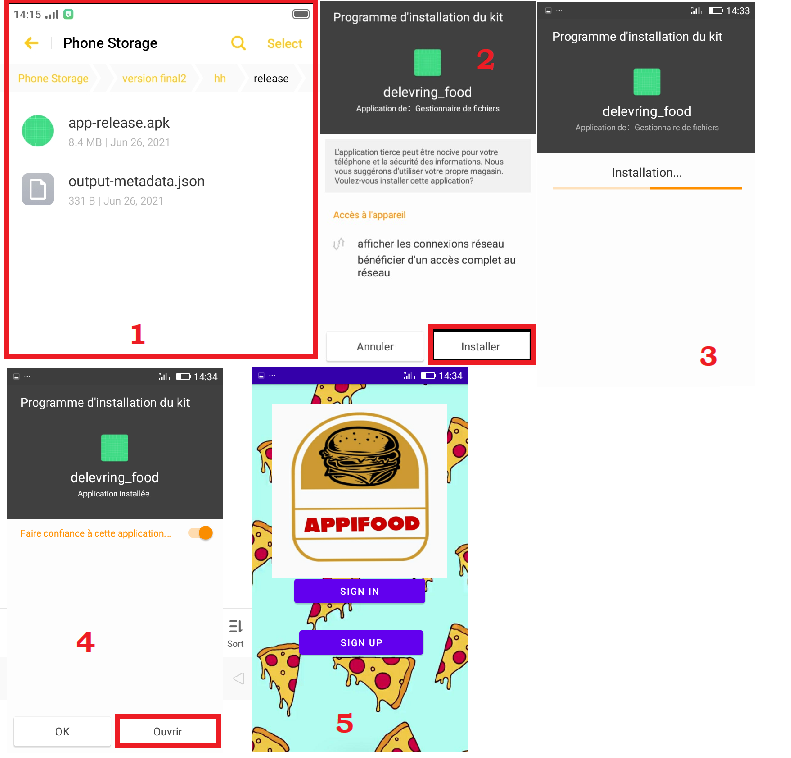
\includegraphics[width=1\linewidth]{images/paint1.png}

\newpage 


\begin{enumerate}
  \item \textbf{Sign in  (Code Source):}
  \begin{lstlisting}
   
  
public class signin extends AppCompatActivity {
 EditText memail,mpassword,phoni;
 Button btn_to_rigister,login_btn;
 FirebaseAuth fauth;
FirebaseDatabase database=FirebaseDatabase.getInstance();
DatabaseReference ref=database.getReference().child("user");
 ProgressBar progressbar;
 @Override
 protected void onCreate(Bundle savedInstanceState) {
 super.onCreate(savedInstanceState);
 setContentView(R.layout.activity_signin);
 memail=findViewById(R.id.login_user);
 mpassword=findViewById(R.id.login_password);
 btn_to_rigister=findViewById(R.id.btn_to_rigister);
 login_btn=findViewById(R.id.login_btn);
 fauth=FirebaseAuth.getInstance();
 progressbar=findViewById(R.id.progressBar);
 phoni=findViewById(R.id.phoni);
 login_btn.setOnClickListener(new View.OnClickListener() {
 @Override
 public void onClick(View v) {
 progressbar.setVisibility(View.VISIBLE);
 ref.addValueEventListener(new ValueEventListener() {
 @Override
public void onDataChange(@NonNull @NotNull
DataSnapshot snapshot) {
 user
u=snapshot.child(phoni.getText().toString()).getValue(user.class);

if(u.getPassword().equals(mpassword.getText().toString()) &&
u.getEmail().equals(memail.getText().toString()) &&
u.getPhone().equals(phoni.getText().toString()) ){

Toast.makeText(signin.this,"ok",Toast.LENGTH_LONG).show();
 loginuser();
 }
else {

Toast.makeText(signin.this,"no",Toast.LENGTH_LONG).show();
 }
 }
 @Override
public void onCancelled(@NonNull @NotNull
DatabaseError error) {
 }
 });
\end{lstlisting}
  
  \newpage
   \item \textbf{Sign Up (Code Source):}
 \begin{lstlisting}
  public class signup extends AppCompatActivity {
 EditText mfullname,mphone,memail,mpassword;
 Button mbtnrigister ,mloginbtn;
 FirebaseAuth fauth;
 ProgressBar progress1;
 FirebaseDatabase database=FirebaseDatabase.getInstance();
DatabaseReference reference=database.getReference().child("user");
 @Override
 protected void onCreate(Bundle savedInstanceState) {
 super.onCreate(savedInstanceState);
 setContentView(R.layout.activity_signup);
 mfullname=findViewById(R.id.fullname);
 database=FirebaseDatabase.getInstance();
 mphone=findViewById(R.id.phone);
 memail=findViewById(R.id.email);
 mpassword=findViewById(R.id.password);
 mbtnrigister=findViewById(R.id.btn_rigister);
 mloginbtn=findViewById(R.id.to_login);
 fauth=FirebaseAuth.getInstance();
 progress1=findViewById(R.id.progress1);
mbtnrigister.setOnClickListener(new View.OnClickListener() {
 @Override
 public void onClick(View v) {
 progress1.setVisibility(View.VISIBLE);
 createuser();
 //createuser();
 /*String email=memail.getText().toString().trim();
 String password=mpassword.getText().toString()
 .trim();
 if(TextUtils.isEmpty(email))
 {
 memail.setError("email is requared");
return;
 }
 if(TextUtils.isEmpty(password))
 {
 mpassword.setError("password is requared");
return;
 }
 if(password.length()<6)
 {
 mpassword.setError("must be > 6 character");
return;
 }
 progress1.setVisibility(View.VISIBLE);
 //firebase /////////////////////////

fauth.createUserWithEmailAndPassword(email,password)
.addOnCompleteListene
r(new OnCompleteListener<AuthResult>() {
 @Override
public void onComplete(@NonNull Task<AuthResult>
task) {
 if(task.isSuccessful())
{
 Toast.makeText(signup.this,"user
created",Toast.LENGTH_SHORT).show();
 startActivity(new
Intent(getApplicationContext(),MainActivity.class));
 }
else
{

Toast.makeText(signup.this,"Erreur"
+task.getException().getMessage(),Toas
t.LENGTH_SHORT).show();
 }
 private void createuser(){
 String fullname=mfullname.getText().toString();
 String email=memail.getText().toString();
 String pss=mpassword.getText().toString();
 String ph=mphone.getText().toString();
 if(TextUtils.isEmpty(fullname))
 {
 Toast.makeText(this,"name is
empty",Toast.LENGTH_LONG).show();
 return;
 }
 if(TextUtils.isEmpty(email))
 {
 Toast.makeText(this,"email is
empty",Toast.LENGTH_LONG).show();
 return;
 }
 if(TextUtils.isEmpty(pss))
 {
 Toast.makeText(this,"password is
empty",Toast.LENGTH_LONG).show();
 return;
 }
 if(TextUtils.isEmpty(ph))
 {
 Toast.makeText(this," phone is
empty",Toast.LENGTH_LONG).show();
 return;
 }
 if(pss.length()<6)
 {
 mpassword.setError("must be > 6 character");
 return;
 }

fauth.createUserWithEmailAndPassword(email,pss)
.addOnCompleteListener(new
OnCompleteListener<AuthResult>() {
 @Override
 public void onComplete(@NonNull Task<AuthResult> task) {
 if(task.isSuccessful())
 {
 user u1=new
user(fullname,email,pss,mphone.getText().toString());

database.getReference().child("user")
.child(mphone.getText().toString()).
setValue(u1);
 Toast.makeText(signup.this,"user
created",Toast.LENGTH_SHORT).show();
 startActivity(new
Intent(getApplicationContext(),act2.class));
 }
 else
 {Toast.makeText(signup.this,"Erreur"
+task.getException().getMessage(),Toas
t.LENGTH_SHORT).show();
 progress1.setVisibility(View.GONE);
 }
 }});

 \end{lstlisting}
  
  
  \newpage
  \item \textbf{Posting Food  (Code Source):}
  \begin{lstlisting}
   public class posting extends AppCompatActivity {
 EditText txt1,txt2,txt3,txtpho;
 Button btnsave,btnshow;
 FirebaseAuth fauth;
 private DatabaseReference refr=
FirebaseDatabase.getInstance().getReference()
.child("category");
 private StorageReference
reference=FirebaseStorage.getInstance()
.getReference();
 private ImageView pic;
 private Uri imageUri;
 ProgressBar progressBar2;
 Food f1 = new Food();
 category c=new category();
 @Override
 protected void onCreate(Bundle savedInstanceState) {
 super.onCreate(savedInstanceState);
 setContentView(R.layout.activity_posting);
 txt1 = findViewById(R.id.txt1);
 txt2 = findViewById(R.id.txt2);
 txt3 = findViewById(R.id.txt3);
 txtpho=findViewById(R.id.txtpho);
 btnsave = findViewById(R.id.btnsave);
 btnshow = findViewById(R.id.btnshow);
 pic = findViewById(R.id.pic);
 progressBar2=findViewById(R.id.progressBar2);
 btnshow.setOnClickListener(new View.OnClickListener() {
 @Override
 public void onClick(View v) {
 Intent galleryintent = new Intent();
 galleryintent.setAction(Intent.ACTION_GET_CONTENT);
 galleryintent.setType("image/*");
 startActivityForResult(galleryintent, 2);
 }
 });
 btnsave.setOnClickListener(new View.OnClickListener() {
 @Override
 public void onClick(View v) {
 /*String name=txt1.getText().toString().trim();
 Integer
quan=Integer.parseInt(txt2.getText().toString()
.trim());
 Integer
price=Integer.parseInt(txt3.getText()
.toString().trim());
 f1.setName(name);
 f1.setQuantite(quan);
 f1.setPrice(price);*/
 if(!txt1.getText().toString().isEmpty() &&
!txt2.getText().toString().isEmpty() &&
!txt3.getText().toString().isEmpty()){
 if(imageUri != null)
 {
 uploadtofirebase(imageUri);
 }
 else {
 Toast.makeText(posting.this, "please select image",
Toast.LENGTH_SHORT).show();
 }}
 //refr.push().setValue(f1);
 //Toast.makeText(this,"sucsses",Toast.LENGTH_LONG)
 .show();
 }
 });
 }
 @Override
 protected void onActivityResult(int requestCode,
 int resultCode,
@Nullable @org.jetbrains.annotations.Nullable Intent data) {
 super.onActivityResult(requestCode, resultCode, data);
 if(requestCode==2 && resultCode==RESULT_OK && data!=null)
 {
 imageUri=data.getData();
 pic.setImageURI(imageUri);
 }
 }
 private void uploadtofirebase(Uri uri){
 StorageReference
fileref=reference.child(System.currentTimeMillis()
+""+getFileExtension(u
ri));
 fileref.putFile(uri).addOnSuccessListener(new
OnSuccessListener<UploadTask.TaskSnapshot>() {
 @Override
 public void onSuccess(UploadTask.TaskSnapshot taskSnapshot) {
 fileref.getDownloadUrl().addOnSuccessListener(new
OnSuccessListener<Uri>() {
 @Override
public void onSuccess(Uri uri) {
 Toast.makeText(posting.this,"uploaded
sucsses",Toast.LENGTH_LONG).show();
 category cc = new
category(txt1.getText().toString(),uri
.toString(),Integer.parseInt(txt3.g
etText().toString()),Integer
.parseInt(txt2.getText().toString()),txtpho.
getText().toString());
 String modelId=refr.push().getKey();
 String
hh=refr.child(txt1.getText().toString()).getKey();
 refr.child(hh).setValue(cc);
 progressBar2.setVisibility(View.GONE);
 }
 });
 }
 }).addOnProgressListener(new
OnProgressListener<UploadTask.TaskSnapshot>() {
 @Override
 public void onProgress(@NonNull @NotNull
UploadTask.TaskSnapshot snapshot) {
 progressBar2.setVisibility(View.VISIBLE);
 }
 }).addOnFailureListener(new OnFailureListener() {
 @Override
 public void onFailure(@NonNull @NotNull Exception e) {
 Toast.makeText(posting.this,"uploaded
failed"+e.getMessage(),Toast.LENGTH_LONG).show();
 }
 });
 }
 private String getFileExtension(Uri mUri)
 {
 ContentResolver cr=getContentResolver();
 MimeTypeMap mime=MimeTypeMap.getSingleton();
 return mime.getExtensionFromMimeType(cr.getType(mUri));
 }
}
  \end{lstlisting}
  
  
   \newpage
  \item \textbf{Class User  (Code Source):}
  \begin{lstlisting}
   public class user {
 private String name;
 private String email;
 private String password;
 private String phone;
 public user(){
 }
 public user(String name,
 String email, String password,
 String phone)
{
 this.name = name;
 this.email = email;
 this.password = password;
 this.phone = phone;
 }
 public String getPhone() {
 return phone;
 }
 public void setPhone(String phone) {
 this.phone = phone;
 }
 public String getEmail() {
 return email;
 }
 public void setEmail(String email) {
 this.email = email;
 }
 public String getName() {
 return name;
 }
 public String getPassword() {
 return password;
 }
 public void setName(String name) {
 this.name = name;
 }
 public void setPassword(String password) {
 this.password = password;
 }
}
  \end{lstlisting}
  
  \newpage
  \item \textbf{Class Food category  (Code Source):}
  \begin{lstlisting}
   public class category {
 private String name;

 private int quantite;
 private String imageUri;
 private int price;
 private String phoneOw;
 public category(){
 }
 public category(String name, String imageUri,int price,int
quantite,String phoneOw) {
 this.name = name;
 this.imageUri = imageUri;
 this.price=price;
 this.quantite=quantite;
 this.phoneOw=phoneOw;
 }
 public String getPhoneOw() {
 return phoneOw;
 }
 public void setPhoneOw(String phoneOw) {
 this.phoneOw = phoneOw;
 }
 public int getQuantite() {
 return quantite;
 }
 public void setQuantite(int quantite) {
 this.quantite = quantite;
 }
 public String getImageUri() {
 return imageUri;
 }
 public void setImageUri(String imageUri) {
 this.imageUri = imageUri;
 }
 public int getPrice() {
 return price;
 }
 public void setPrice(int price) {
 this.price = price;
 }
 public String getName() {
 return name;
 }
 public void setName(String name) {
 this.name = name;
 }
}
  \end{lstlisting}
  
  \newpage
  \item \textbf{Class Main Interface  (Code Source):}
  \begin{lstlisting}
  public class act2 extends AppCompatActivity {
 TextView txtviewjdid;
 @Override
 protected void onCreate(Bundle savedInstanceState) {
 super.onCreate(savedInstanceState);
 setContentView(R.layout.activity_act2);
 Intent mm=getIntent();
 String h=mm.getStringExtra("idphone");
 txtviewjdid=(TextView)findViewById(R.id.txtviewjdid);
 txtviewjdid.setText(h);
 }
 public void onclickpos(View view) {
 Intent i=new Intent(act2.this,posting.class);
 startActivity(i);
 }
 public void onclickorder(View view) {
 Intent i2=new Intent(act2.this,home.class);
 startActivity(i2);
 }
 public void onclickvoir(View view) {
 Intent i3=new Intent(act2.this,MainActivity2.class);
 i3.putExtra("gggg",txtviewjdid.getText().toString());
 startActivity(i3);
 }
 public void onclickacceptcommande(View view) {
 Intent i4=new Intent(act2.this,acceptcommande.class);
 i4.putExtra("ffff",txtviewjdid.getText().toString());
 startActivity(i4);
 }
}
  \end{lstlisting}
  
  
   \newpage
  \item \textbf{Class Home activity  (Code Source):}
  \begin{lstlisting}
  public class MainActivity2 extends AppCompatActivity {
TextView txtquant,txtquanttotal,name;
 private DatabaseReference refr2=
FirebaseDatabase.getInstance()
.getReference().child("commande");
private DatabaseReference refr1=
FirebaseDatabase.getInstance()
.getReference().child("category");
 private DatabaseReference refr3=
FirebaseDatabase.getInstance()
.getReference().child("commandeaccepter");
 Button btnvalider;
category cm=new category();
 FirebaseDatabase database;
 DatabaseReference commande;
 RecyclerView recycle1;
 RecyclerView.LayoutManager LayoutManager;
 @Override
 protected void onCreate(Bundle savedInstanceState) {
 super.onCreate(savedInstanceState);
 setContentView(R.layout.activity_main2);
 database=FirebaseDatabase.getInstance();
 commande=database.getReference("commande");
txtquant=findViewById(R.id.txtquant);
txtquanttotal=findViewById(R.id.txtquanttotal);
name=findViewById(R.id.name);
 recycle1=(RecyclerView)findViewById(R.id.recycler1);
 recycle1.setHasFixedSize(true);
 LinearLayoutManager layoutManager = new LinearLayoutManager
(this);
 layoutManager= new LinearLayoutManager(this);
 recycle1.setLayoutManager(layoutManager);
 Intent i3 = getIntent();
 String phoneownerr=i3.getStringExtra("gggg");
 if(!phoneownerr.isEmpty()){
 loadmenu();}
 }
 private void loadmenu() {
 Intent i3 = getIntent();
 String phoneownerr=i3.getStringExtra("gggg");
 FirebaseRecyclerAdapter<commande, menuviewholder> adapter=new
FirebaseRecyclerAdapter<com.example
.delevring_food.commande,
menuviewholder>(commande.class,
R.layout.cmd,menuviewholder.class,commande
.child(phoneownerr.toString())) {
 @Override
 protected void populateViewHolder(menuviewholder
menuviewholder, com.example.
delevring_food.commande commande, int i) {
 menuviewholder.name.setText(commande.getName());

menuviewholder.txtquant
.setText(String.valueOf(commande
.getQuantite()));

menuviewholder.txtquanttotal
.setText(String.valueOf(commande.getQuantitet
otal()));
 com.example.delevring_food.commande
clickitem=commande;
 menuviewholder.setItemclicklistener(new
ItemClickListener() {
 @Override
public void onClick(View view, int position,
boolean isLongClick) {
 AlertDialog alertDialog=new
AlertDialog.Builder(MainActivity2.this)
.setIcon(android.R.drawable.ic_dia
log_alert).setTitle("are you sure")
.setMessage("to accepter this
request").setPositiveButton("accepte", new
DialogInterface.OnClickListener() {
 @Override
 public void onClick(DialogInterface dialog,
int which) {
 Integer a1=clickitem.getQuantitetotal();
Integer a2=clickitem.getQuantite();
 Integer a=a1-a2;

Toast.makeText(MainActivity2.this,""
+a,Toast.LENGTH_LONG).show();
 HashMap hashMap = new HashMap();
hashMap.put("quantite",a);
refr1.child(clickitem.getName().toString())
.updateChildren(hashMap).addOn
SuccessListener(new OnSuccessListener() {
 @Override
public void onSuccess(Object o) {

Toast.makeText(MainActivity2.this, "sucsses",
Toast.LENGTH_LONG)
.show();
 }
 });
Toast.makeText(MainActivity2.this,"okkkkk",
Toast.LENGTH_LONG).show();

commande cm2=new commande();
cm2.setName(clickitem.getName());
 cm2.setQuantite(clickitem.getQuantite());
 cm2.setPhoneOw(phoneownerr);

refr3.child(clickitem.getPhoneOw().toString())
.push().setValue(cm2);
 }
 }).setNegativeButton("delete", new
DialogInterface.OnClickListener() {
 @Override
public void onClick(DialogInterface dialog,
int which) {

refr2.child(phoneownerr).child(getRef(position)
.getKey()).removeValue();

 }
}).show();}});};
 recycle1.setAdapter(adapter);
 }}
  \end{lstlisting}
  
  \newpage
  \item \textbf{Class Home Food  (Code Source):}
  \begin{lstlisting}
  public class home extends AppCompatActivity {
 private AppBarConfiguration mAppBarConfiguration;
 private ActivityHomeBinding binding;
 FirebaseDatabase database;
 DatabaseReference category;
 RecyclerView recycle_menu;
 RecyclerView.LayoutManager LayoutManager;
 MenuItem nav_logout;
 @Override
 protected void onCreate(Bundle savedInstanceState) {
 super.onCreate(savedInstanceState);
 binding = ActivityHomeBinding.
 inflate(getLayoutInflater());
 setContentView(binding.getRoot());
///////////////////
 
 /////firebase
 database=FirebaseDatabase.getInstance();
 category=database.getReference("category");
 TextView txtfullname;
 setSupportActionBar(binding.appBarHome.toolbar);

 DrawerLayout drawer = binding.drawerLayout;
 NavigationView navigationView = binding.navView;
 
 mAppBarConfiguration = new AppBarConfiguration.Builder(
 R.id.nav_home, R.id.nav_gallery, R.id.nav_slideshow)
 .setDrawerLayout(drawer)
 .build();
 NavController navController = Navigation.findNavController(this,
R.id.nav_host_fragment_content_home);
 NavigationUI.setupActionBarWithNavController(
 this, navController,
mAppBarConfiguration);
 NavigationUI.setupWithNavController(
 navigationView,
navController);
 //////
 View headerview=navigationView.getHeaderView(0);
 txtfullname=(TextView)headerview
 .findViewById(R.id.txtfullname);
 //txtfullname.setText(common.currentuser.getName());
 ////load menu
 recycle_menu=(RecyclerView)findViewById(R
 .id.recycle_menu);
 recycle_menu.setHasFixedSize(true);
 LinearLayoutManager layoutManager = new LinearLayoutManager
(this);
 layoutManager= new LinearLayoutManager(this);
 recycle_menu.setLayoutManager(layoutManager);
 loadmenu();
 }
 private void loadmenu() {
 FirebaseRecyclerAdapter<category, menuviewholder> adapter=new
FirebaseRecyclerAdapter<com.example
.delevring_food.model.category,
menuviewholder>(category.class,R
.layout.menu_item,menuviewholder.class,ca
tegory) {
 @Override
 protected void populateViewHolder(menuviewholder
menuviewholder, com.example.delevring_food.model.category category, int
i) {
 menuviewholder.txtmenuname.setText(category
 .getName());

Picasso.with(getBaseContext()).load(category
.getImageUri())
 .into(menuviewholder.imageview);

menuviewholder.txtprice
.setText(String.valueOf(category.getPrice()));

menuviewholder.txtquantite
.setText(String.valueOf(category.getQuantite())
);
 menuviewholder.txtphomenu
 .setText(category.getPhoneOw());
 com.example.delevring_food.model.category
clickitem=category;
 menuviewholder.setItemclicklistener(new
ItemClickListener() {
 @Override
public void onClick(View view, int position, boolean
isLongClick) {

Toast.makeText(home.this,""
+clickitem.getName(),Toast.LENGTH_SHORT).show(
);
 Intent intent=new
Intent(home.this,detailsF.class);
 //FirebaseRecyclerAdapter<category,
menuviewholder> adapter=null;



intent.putExtra("FoodId",clickitem
.getName().toString());

intent.putExtra("Foods",menuviewholder.txtprice
.getText().toString());

intent.putExtra("Foodsquan",menuviewholder
.txtquantite.getText().toString
());

intent.putExtra("ownerphone",menuviewholder
.txtphomenu.getText().toString
());

intent.putExtra("key",category.getImageUri());
 
 startActivity(intent);
 }});};
 recycle_menu.setAdapter(adapter);}
 @Override
 public boolean onCreateOptionsMenu(Menu menu) {
 getMenuInflater().inflate(R.menu.home, menu);
 return true;}
 @Override
 public boolean onSupportNavigateUp() {
 NavController navController = Navigation.findNavController(this,
R.id.nav_host_fragment_content_home);
 return NavigationUI.navigateUp(navController,
mAppBarConfiguration)
 || super.onSupportNavigateUp();
 }
}
  \end{lstlisting}
  
  \newpage
  \item \textbf{Class Details Food  (Code Source) :}
  \begin{lstlisting}
  public class detailsF extends AppCompatActivity {
TextView food_name,food_price,
txtquan,txtviewtel,inputiquan,txtnewview;
ImageView img_food;
Button btncommande;
 FirebaseAuth fauth;
 private DatabaseReference refr=
FirebaseDatabase.getInstance().getReference()
.child("commande");
 private StorageReference reference=
FirebaseStorage.getInstance().getReference();
 private DatabaseReference refr1=
FirebaseDatabase.getInstance().getReference()
.child("category");
 private StorageReference reference1=
FirebaseStorage.getInstance().getReference();
 commande cm=new commande();
EditText txtviewnewquan;
 @Override
 protected void onCreate(Bundle savedInstanceState) {
 super.onCreate(savedInstanceState);
 setContentView(R.layout.activity_details_f);
 food_name = findViewById(R.id.food_name);
 img_food = findViewById(R.id.img_food);
 food_price=findViewById(R.id.food_price);
 btncommande=findViewById(R.id.btncommande);
 txtviewtel=findViewById(R.id.txtviewtel);
 txtquan=findViewById(R.id.txtquan);
 txtviewnewquan=findViewById(R.id.txtviewnewquan);
 txtnewview=findViewById(R.id.txtnewview);
 //inputiquan.findViewById(R.id.inputiquan);
 Intent i = getIntent();
 Bundle extras=getIntent().getExtras();
 Uri ii=Uri.parse(extras.getString("key"));
 String n = i.getStringExtra("FoodId");
 String n2=i.getStringExtra("Foods");
 String n3=i.getStringExtra("Foodsquan");
 String s4=i.getStringExtra("ownerphone");

Picasso.with(getBaseContext())
.load(Uri.parse(getIntent().getStringExtra(
"key"))).into(img_food);

 food_name.setText(n);
 food_price.setText(n2);
 txtquan.setText(n3);
 txtviewtel.setText(s4);
///to mainactivity2
Intent intenti=new Intent(detailsF.this,MainActivity2.class);
 intenti.putExtra("phoneowner",txtviewtel
 .getText().toString());
/////
 btncommande.setOnClickListener(new View.OnClickListener() {
 @Override
 public void onClick(View v) {
 String name = food_name.getText().toString()
 .trim();
 Integer quan =
Integer.parseInt(txtquan.getText().toString()
.trim());
 Integer price =
Integer.parseInt(food_price.getText()
.toString().trim());
 String ownrp = txtviewtel.getText().toString().trim();
 if(!name.isEmpty() &&
!String.valueOf(quan).toString().
isEmpty() &&
!String.valueOf(price).toString()
.isEmpty() && !ownrp.isEmpty() &&
!txtnewview.getText().toString()
.isEmpty() &&
!txtviewnewquan.getText().toString()
.isEmpty())
 {
 if (quan >=
Integer.parseInt(txtviewnewquan.getText()
.toString())) {
 //quan = quan -
(Integer.parseInt(txtviewnewquan.getText()
.toString().trim()));

 AlertDialog alertDialog=new
AlertDialog.Builder(detailsF.this)
.setIcon(android.R.drawable.ic_dialog_a
lert).setTitle("are you sure")
.setMessage("to commande this
food").setPositiveButton("yes",
new DialogInterface.OnClickListener() {
 @Override
public void onClick(DialogInterface dialog, int
which) {
 cm.setName(name);
 cm.setPrice(price);
cm.setPhoneOw(txtnewview.getText().toString());

cm.setQuantite(Integer.parseInt(txtviewnewquan
.getText().toString()));
 cm.setQuantitetotal(quan);
//refr.push().setValue(cm);

refr.child(ownrp.toString()).push().setValue(cm);
 Toast.makeText(detailsF.this, "sucsses",
Toast.LENGTH_LONG).show();

Toast.makeText(detailsF.this,"okkkkk",
Toast.LENGTH_LONG).show();
 }
 }).setNegativeButton("no", new
DialogInterface.OnClickListener() {
 @Override
public void onClick(DialogInterface dialog, int
which) {

Toast.makeText(detailsF.this,"cancel",
Toast.LENGTH_LONG).show();
 }
 }).show();
 }
 else
 {
 Toast.makeText(detailsF.this,"
 failed the quantity <
desponible",Toast.LENGTH_LONG).show();
 }}
 else
 {

Toast.makeText(detailsF.this,"failed",
Toast.LENGTH_LONG).show();
 }});
 
  
   \end{lstlisting}
\end{enumerate}